% -----------------------------------------------------
% -------- BAYSIS - Selected as Jam Initiator ---------
% -----------------------------------------------------
\subsection{Congestion - Accidents categorizes as Jam Initiator}
\label{analysis_processing_correlation_baysis_initiator}
The correlation matrix table for the congestion - accident dataset, which are classified as \textit{Jam Initiator} (see \cref{table:appendix_correlation_matrix_matched_cramers}) is visual presented in \cref{img:correlation_matrix_selected_initiator_cramers} showing the the correlation of each variable combination. When visual analyzing \cref{img:correlation_matrix_matched_cramers} and checking the guidelines for a strong correlation in reference to the applied coefficient (identifiable with \cref{table:appendix_coefficient_matrix_matched}) we get a list of strongly correlated variable combinations (see \cref{tbl:correlation_list_baysis_initiator}). Since the focus of the thesis are the correlations between accidents and jams, these are only collected from the bottom-left rectangle of the matrix, where the congestion and accidents variables intersect. Correlations of the kind congestion - congestion or accident - accident are not considered.
\begin{table}[ht!]
	\centering
	\begin{tabular}{c|l}  
		\toprule
		\textit{Category} & \textit{Strong} \\
		\midrule
		Strasse & TMax, TAvg, SMax, SAvg, Cov, TLCar \\ 
 		Kat & TMax, TAvg, SMax, SAvg \\ % -> Strasse
 		Typ & SAvg, TDist, Cov \\ % -> Strasse
 		%Betei & \\
 		UArt1 & TMax, TAvg, SMax, SAvg, TDist, Cov, TLCar \\
 		%UArt2 & \\ % -> Strasse
 		AUrs1 & TMax, TAvg, SMax, SAvg, TDist, Cov, TLHGV \\ % -> Strasse
 		AUrs2 & TMax, TAvg, SAvg, TDist \\
 		AufHi & TMax, TAvg, TDist, Cov \\
 		%Alkoh & \\
 		Char1 & TDist \\ % -> Strasse
 		%Char2 & \\
 		%Bes1 & \\
 		Lich1 & TDist \\
 		Lich2 & TDist \\ % -> Strasse
 		Zust1 & Cov \\
 		Zust2 & TAvg, SAvg \\ % -> Strasse
 		%Fstf & \\
 		%WoTag & \\
 		%FeiTag & \\
 		Month & SMax, Cov, TLHGV \\ % -> Strasse
 		\bottomrule
	\end{tabular}
	\caption{List of incident variables and their strong correlated congestion variable from the congestion-accident matched data which are classified as \textit{Jam Initiator}}
	\label{tbl:correlation_list_baysis_initiator}
\end{table}
Next we need to verify that the correlation is significant and what the correlation predicates. Therefore each correlation will be evaluated with the Post Hoc test, defined in \cref{correlation_posthoc}. \secintroend{baysis}{initiator}
\begin{figure}[!ht]
	\centering
	\makebox[\textwidth][c]{%
		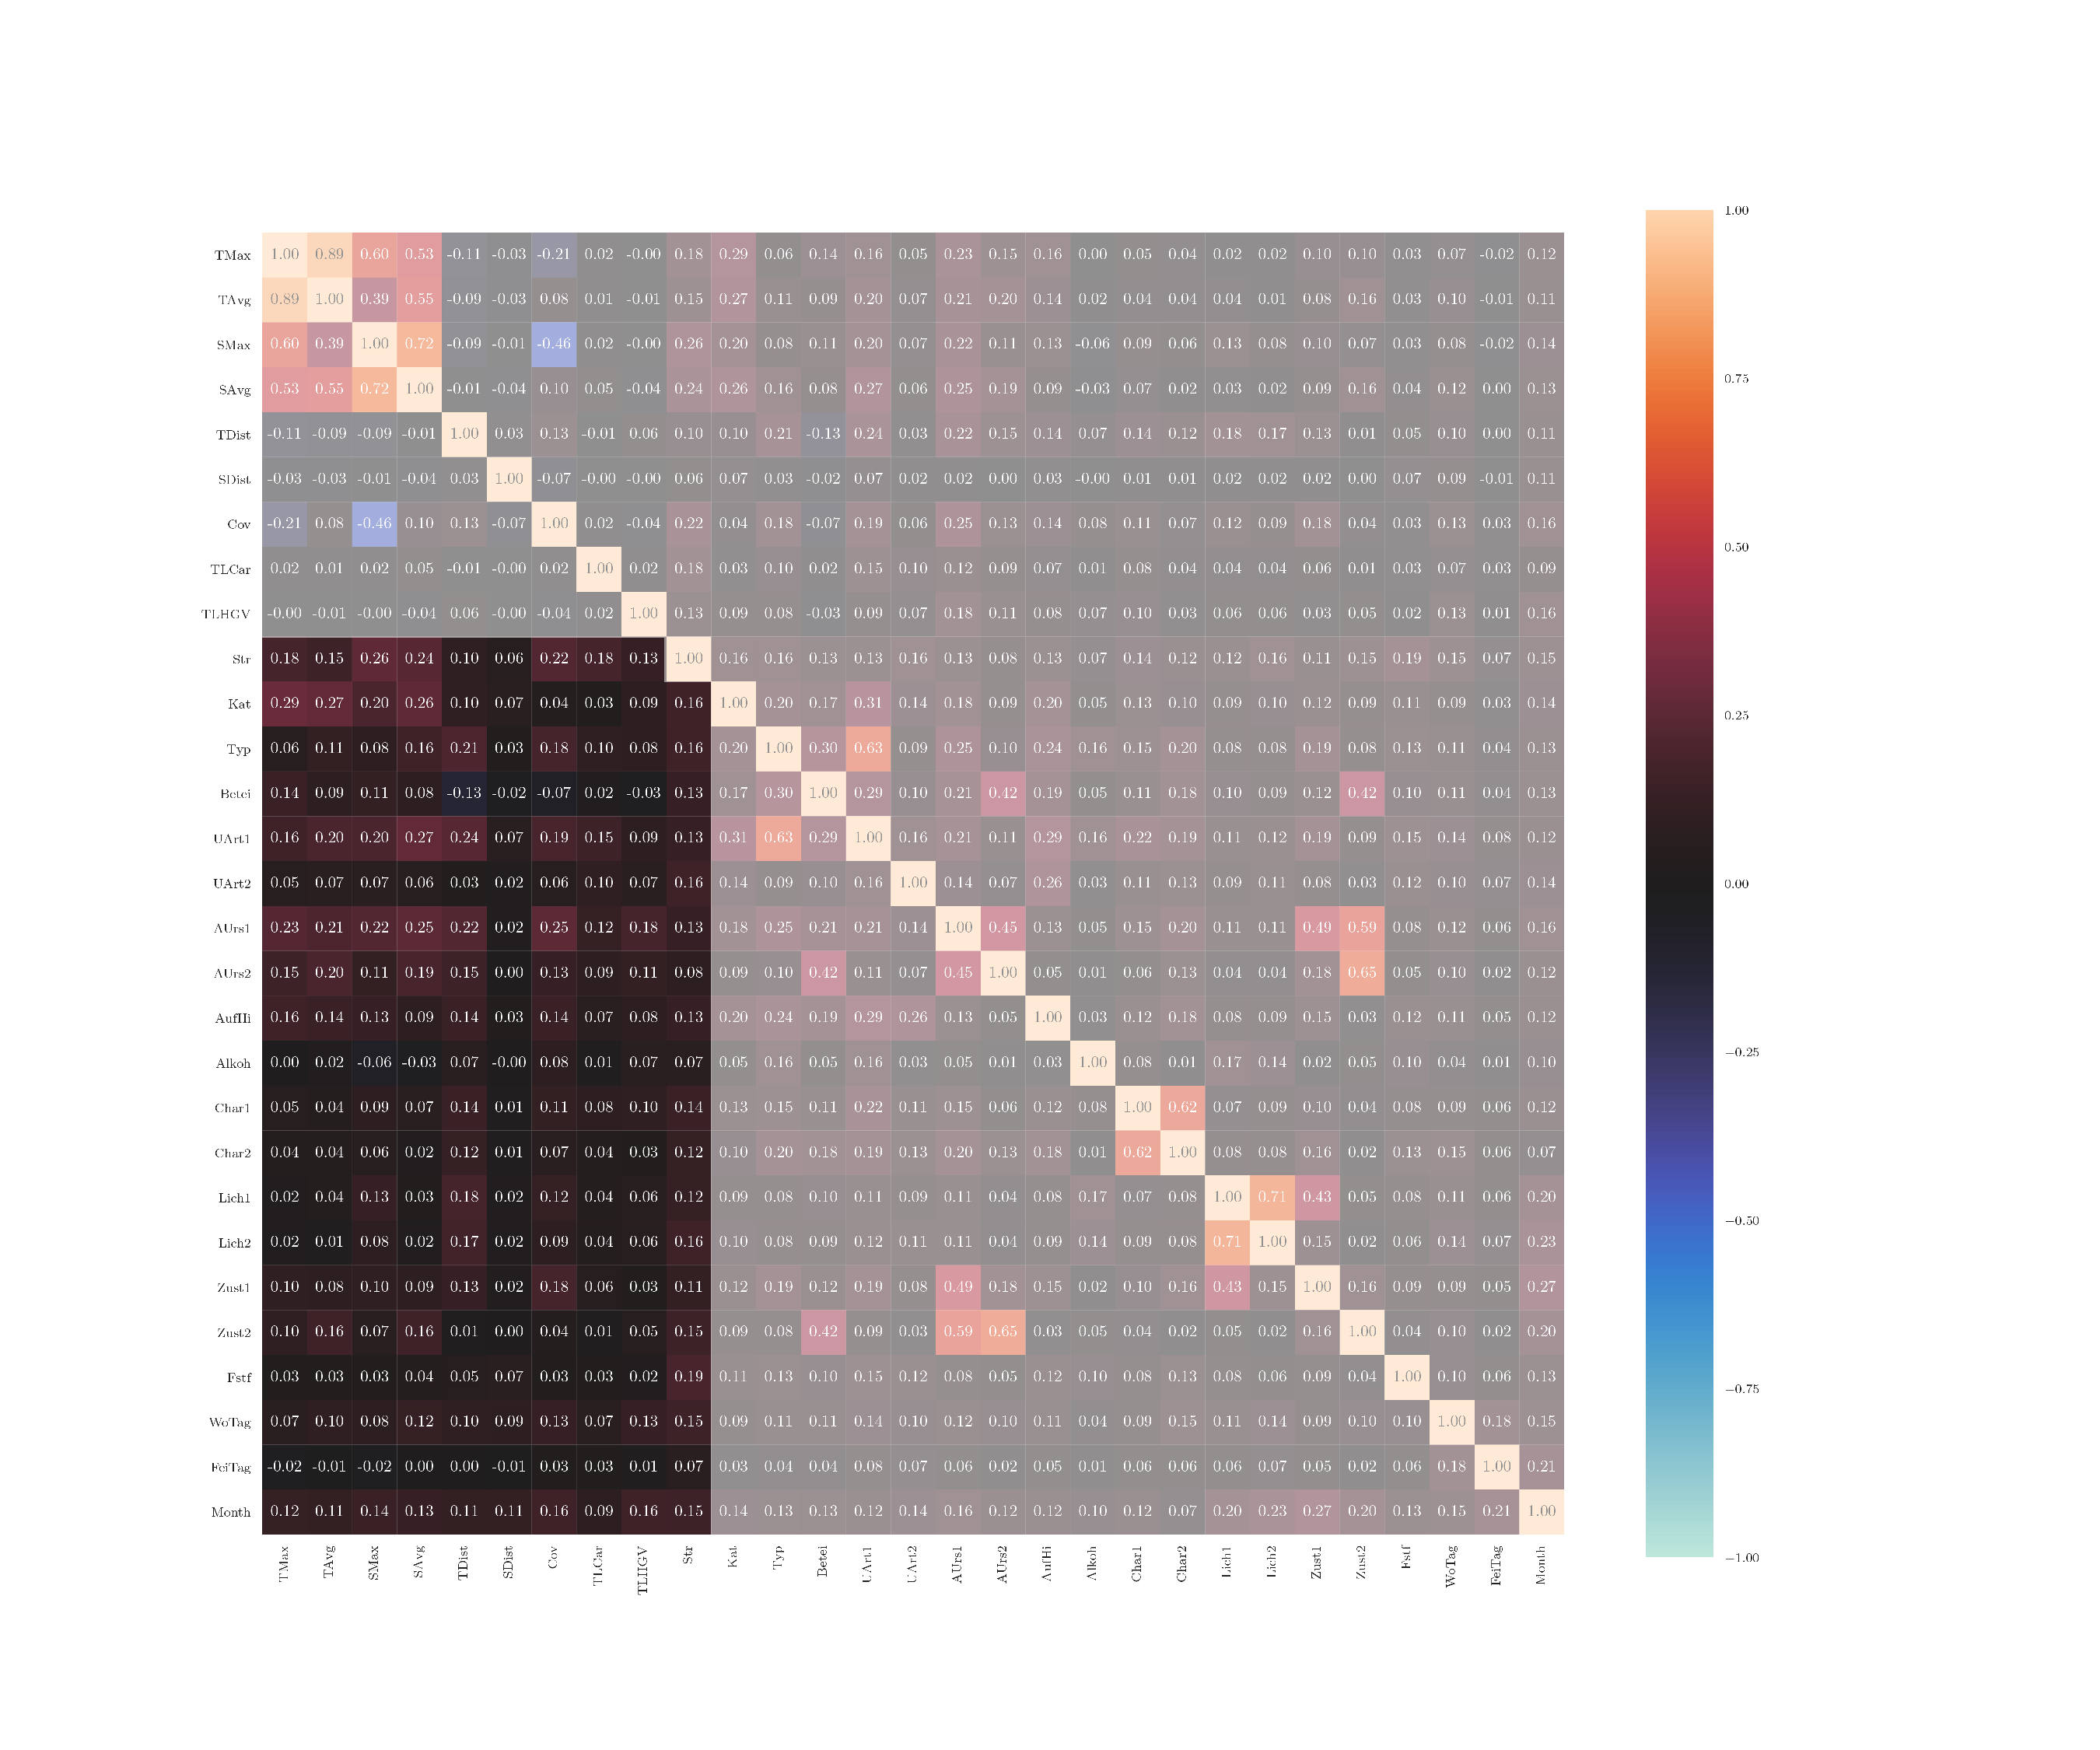
\includegraphics[width=1.4\textwidth, trim=0cm 2.5cm 6cm 3cm]{CorrAnalysis/data/BAYSIS/03_selected_01_startJam/plots/baysis_selected_corr_cramers_edited}%
	}
	\caption{Correlation matrix for congestion-accident matched data classified as \textit{Jam Initiator} and calculated with $V$, $\eta$, $\tau$, $r_{pq}$, $r$}
	\label{img:correlation_matrix_selected_initiator_cramers}
\end{figure}

% --------------------------
% -------- Strasse ---------
% --------------------------
\centerheading{Strasse}
\varintronosigmul{Kat}{\textit{Strasse} - \textit{TMax}, \textit{Strasse} - \textit{TAvg}, \textit{Strasse} - \textit{SMax}, \textit{Strasse} - \textit{SAvg}, \textit{Strasse} - \textit{Cov} and \textit{Strasse}-\textit{TLCar}}

% ----------------------
% -------- Kat ---------
% ----------------------
\centerheading{Kat}
\varintrowithsam{baysis}{Kat} \varintronosigmul{Kat}{\textit{Kat}-\textit{SMax} and \textit{Kat}-\textit{SAvg}}

% ###########################################
\groupintrosig{Kat}{TMax}{0.0001}{baysis}{initiator}
\begin{table}[ht!]
    \tiny
	\centering
	\begin{tabular}{rrrr}
		\toprule  
  		  & 1 & 2 & 3 \\ 
  		\midrule    
        2 & \red{0.00} &  &  \\ 
        3 & \red{0.00} & \red{0.00} &  \\ 
        7 & \red{0.00} & \red{0.00} & \red{0.00} \\ 
 		\bottomrule
	\end{tabular}
    \caption{Pairwise Wilcoxon $T$-test for \textit{Kat} and \textit{Maximal Temporal Extent} (Jam Initiator)}
    \label{tbl:wilcoxon_baysis_initiator_Kat_TMax}
\end{table}
It shows that all groups have significant differences and therefore \textit{TMax} has a general trend.
% #### START: Table and Plot
\begin{figure}[ht!]
	\centering
	\begin{minipage}{0.5\textwidth}
		\tiny
		\setlength{\tabcolsep}{4pt}
		\centering
		\begin{tabular}{c|c|c|c|c|c|c|c}
			\toprule
			Group & $n$ & $\bar{x}$ & $\sigma$ & $\tilde{x}$ & $min$ & $max$ & $\Delta$ \\
			\midrule
            1 & 29  & 290.07 & 190.59 & 255.00 & 27 & 864  & 837 \\ 
            2 & 144 & 156.23 & 119.44 & 120.00 & 9  & 657  & 648 \\ 
            3 & 422 & 120.18 & 103.92 & 99.00  & 9  & 1116 & 1107 \\ 
            7 & 181 & 103.13 & 143.89 & 75.00  & 9  & 1341 & 1332 \\ 
			\bottomrule
			% \bar{x} - sum = 669.61, mean = 167.40
			% \sigma - sum = 557.84, mean = 139.46
			% \tilde{x}
			%
            % 156+121+103 / 3 = 126
            % diff 126,290 = 164
            % mean diff 156,121,103 = 26
		\end{tabular}
		\subcaption[second caption.]{Table of all descriptives}\label{tbl:descriptives_baysis_initiator_Kat_TMax}
	\end{minipage}%
	\begin{minipage}{0.55\textwidth}
		\pgfplotstableread[col sep=comma]{
			road, count, mean, median, sd, min, max, delta
            1 , 29  , 290.07 , 190.59 , 255 , 27 , 864  , 837 
            2 , 144 , 156.23 , 119.44 , 120 , 9  , 657  , 648 
            3 , 422 , 120.18 , 103.92 , 99  , 9  , 1116 , 1107 
            7 , 181 , 103.13 , 143.89 , 75  , 9  , 1341 , 1332 
		}\data
        \pgfplotstablesort[sort key=mean, sort cmp=float >]{\datasorted}{\data}
        \tiny
        \centering
        \descplotfigwithavg{\datasorted}{167}{139}{3}{4.7}
		\subcaption[second caption.]{Plot of descriptives $\bar{x}$, $\sigma$ and $\tilde{x}$}\label{fig:descriptives_baysis_initiator_Kat_TMax}
	\end{minipage}%
	\caption{Group descriptives of \textit{Kat} and \textit{Maximal Temporal Extent} (Jam Initiator)}
	%\vspace{-8mm}
\end{figure}
% #### END: Table and Plot
The significant descriptives from \cref{tbl:descriptives_baysis_initiator_Kat_TMax,fig:descriptives_baysis_initiator_Kat_TMax} present increasing means from accidents with property damage to deathly accidents. Therefore it can be interpreted that the maximal temporal jam length significant increases with the gravity of the accident. Also the difference of group 1 to group 2, 3 and 7 is considerable, which means that the accidents with deaths are associated with 164\,min longer jams, than others. The groups 2, 3 and 7 differ on by 26\,min on average. 
\groupintrosig{Kat}{TAvg}{0.0087}{baysis}{initiator} 
\begin{table}[ht!]
	\tiny
	\centering
    \begin{tabular}{rrrr}
        \toprule
          & 1 & 2 & 3 \\ 
        \midrule
        2 & \red{0.00} &  &  \\ 
        3 & \red{0.00} & \red{0.01} &  \\ 
        7 & \red{0.00} & \red{0.00} & \red{0.00} \\ 
        \bottomrule
    \end{tabular}
	\caption{Pairwise Wilcoxon $T$-test for \textit{Kat} and \textit{Average Temporal Extent} (Jam Initiator)}
	\label{tbl:wilcoxon_baysis_initiator_Kat_TAvg}
\end{table}
It shows that all groups have significant differences and therefore \textit{TAvg} has a general trend.
% #### START: Table and Plot
\begin{figure}[ht!]
	\centering
	\begin{minipage}{0.5\textwidth}
		\tiny
		\setlength{\tabcolsep}{4pt}
		\centering
		\begin{tabular}{c|c|c|c|c|c|c|c}
			\toprule
			Group & $n$ & $\bar{x}$ & $\sigma$ & $\tilde{x}$ & $min$ & $max$ & $\Delta$ \\
			\midrule
            1 & 29  & 148.76 & 90.65 & 144.0 & 20 & 376 & 356 \\ 
            2 & 144 & 80.91  & 67.52 & 61.5  & 7  & 426 & 419 \\ 
            3 & 422 & 63.75  & 51.27 & 53.0  & 5  & 469 & 464 \\ 
            7 & 181 & 53.61  & 80.96 & 39.0  & 4  & 920 & 916 \\ 
			\bottomrule
			% \bar{x} - sum = 347.03, mean = 86.75
			% \sigma - sum = 290.40, mean = 72.6
			% \tilde{x}
			%
            % 80+63+53 / 3 = 65
            % diff 148,65 = 83
            % mean diff 80,63,53 = 10
		\end{tabular}
		\subcaption[second caption.]{Table of all descriptives}\label{tbl:descriptives_baysis_initiator_Kat_TAvg}
	\end{minipage}%
	\begin{minipage}{0.55\textwidth}
		\pgfplotstableread[col sep=comma]{
			road, count, mean, median, sd, min, max, delta
            1 , 29  , 148.76 , 90.65 , 144.0 , 20 , 376 , 356 
            2 , 144 , 80.91  , 67.52 , 61.5  , 7  , 426 , 419 
            3 , 422 , 63.75  , 51.27 , 53.0  , 5  , 469 , 464 
            7 , 181 , 53.61  , 80.96 , 39.0  , 4  , 920 , 916 
		}\data
        \pgfplotstablesort[sort key=mean, sort cmp=float >]{\datasorted}{\data}
        \tiny
        \centering
        \descplotfigwithavg{\datasorted}{86}{72}{3}{4.7}
		\subcaption[second caption.]{Plot of descriptives $\bar{x}$, $\sigma$ and $\tilde{x}$}\label{fig:descriptives_baysis_initiator_Kat_TAvg}
	\end{minipage}%
	\caption{Group descriptives of \textit{Kat} and \textit{Average temporal Extent} (Jam Initiator)}
	%\vspace{-8mm}
\end{figure}
% #### END: Table and Plot
The significant descriptives from \cref{tbl:descriptives_baysis_initiator_Kat_TAvg,fig:descriptives_baysis_initiator_Kat_TAvg} present increasing means from accidents with property damage to deathly accidents. Therefore it can be interpreted that the average temporal jam length significant increases with the gravity of the accident. Also the difference of group 1 to group 2, 3 and 7 is considerable, which means that the accidents with deaths are associated with 83\,min longer jams, than others. The groups 2, 3 and 7 differ on by 10\,min on average. 
\begin{figure}[ht!]
	\pgfplotstableread[col sep=comma]{
		Kat, meanTMax, meanTAvg  
		1 , 290.07 , 148.76
		2 , 156.23 , 80.91 
		3 , 120.18 , 63.75 
		7 , 103.13 , 53.61 
	}\data
    \pgfplotstablesort[sort key=meanTAvg, sort cmp=float >]{\datasorted}{\data}
    \tiny
    \centering
	\barplotdouble{\datasorted}{meanTMax}{meanTAvg}{$\bar{x}_{TMax}$}{$\bar{x}_{TAvg}$}
	\caption{Comparison of descriptives $\bar{x}_{TMax}$ and $\bar{x}_{TAvg}$ (\textit{TMax/TAvg} by \textit{Kat})}
	\label{fig:baysis_initiator_meancomparison_Kat_temporal}
	%\vspace{-8mm}
\end{figure}
When comparing the mean values of the maximal and average (temporal) extend (shown in \cref{fig:baysis_initiator_meancomparison_Kat_temporal}) it becomes clear that the average is significantly lower than the maximum, which is to be expected. It also shows, that the difference between the groups are similar in the maximal and average extend. In can be described that they follow the same tend, that the jam duration significant increases with the gravity of the accident.

% ----------------------
% -------- Typ ---------
% ----------------------
\centerheading{Typ}
\varintrowithsam{baysis}{Typ} \varintronosigsing{Typ}{Cov}

% ############################################
\groupintrosig{Typ}{TDist}{0.0264}{baysis}{initiator}
\begin{table}[ht!]
	\tiny
	\centering
    \begin{tabular}{rrrrrr}
        \toprule
        & 1 & 3 & 4 & 5 & 6 \\ 
        \midrule
        3 & \red{0.05} &  &  &  &  \\ 
        % 4 & 1.00 & 0.38 &  &  &  \\ 
        % 5 & 0.96 & 1.00 & 0.96 &  &  \\ 
        6 & \red{0.00} & 0.96 & 0.51 & 1.00 &  \\ 
        7 & 1.00 & \red{0.04} & 1.00 & 0.96 & \red{0.01} \\ 
        \bottomrule
    \end{tabular}
    \caption{Pairwise Wilcoxon $T$-test for \textit{Typ} and \textit{Temporal Distance} (Jam Initiator), see \cref{tbl:wilcoxon_baysis_initiator_Typ_TDist_complete} for complete table}
    \label{tbl:wilcoxon_baysis_initiator_Typ_TDist}
\end{table}
It shows that group 6 differs significantly from group 1 and group 7 from 6, but there is no distinctive general trend.
% #### START: Table and Plot
\begin{figure}[ht!]
	\centering
	\begin{minipage}{0.5\textwidth}
		\tiny
		\setlength{\tabcolsep}{4pt}
		\centering
		\begin{tabular}{c|c|c|c|c|c|c|c}
			\toprule
			Group & $n$ & $\bar{x}$ & $\sigma$ & $\tilde{x}$ & $min$ & $max$ & $\Delta$ \\
			\midrule
            1 & 181 & 11.40 & 6.38 & 10.00 & 1  & 24 & 23 \\ 
            3 & 24  & 7.67  & 6.06 & 7.00  & 1  & 22 & 21 \\ 
            6 & 495 & 9.21  & 5.88 & 8.00  & 0  & 24 & 24 \\ 
            7 & 70  & 12.27 & 7.09 & 11.00 & 0  & 24 & 24 \\ 
			\bottomrule
			% \bar{x} - sum = 40.55, mean = 10.13
			% \sigma - sum = 25.41, mean = 6.35
			% \tilde{x}
		\end{tabular}
		\subcaption[second caption.]{Table of all descriptives}\label{tbl:descriptives_baysis_initiator_Typ_TDist}
	\end{minipage}%
	\begin{minipage}{0.55\textwidth}
		\pgfplotstableread[col sep=comma]{
			road, count, mean, median, sd, min, max, delta
            1 , 181 , 11.40 , 6.38 , 10 , 1 , 24 , 23 
            3 , 24  , 7.67  , 6.06 , 7  , 1 , 22 , 21 
            6 , 495 , 9.21  , 5.88 , 8  , 0 , 24 , 24 
            7 , 70  , 12.27 , 7.09 , 11 , 0 , 24 , 24 
		}\data 
        \pgfplotstablesort[sort key=mean, sort cmp=float >]{\datasorted}{\data}
        \tiny
        \centering
        \descplotfigwithavg{\datasorted}{10.13}{6.35}{3}{3.7}
		\subcaption[second caption.]{Plot of descriptives $\bar{x}$, $\sigma$ and $\tilde{x}$}\label{fig:descriptives_baysis_initiator_Typ_TDist}
	\end{minipage}%
	\caption{Group descriptives of \textit{Kat} and \textit{Temporal Distance}}
	%\vspace{-8mm}
\end{figure}
% #### END: Table and Plot
The significant descriptives in \cref{tbl:descriptives_baysis_initiator_Typ_TDist,fig:descriptives_baysis_initiator_Typ_TDist} show that the groups 1 and 7 have higher means than group 3 and 6. Therefore it can be interpreted that temporal distance of \textit{driving} and \textit{other} accidents (average of 12\,min) is substantial higher than for \textit{merging}, \textit{crossing} and \textit{straight traffic} accidents (average of 8\,min).

% ------------------------
% -------- UArt1 ---------
% ------------------------
\centerheading{UArt}
\varintrowithsam{baysis}{UArt} \varintronosigmul{UArt}{\textit{UArt1} - \textit{TAvg}, \textit{UArt1} - \textit{SMax}, \textit{UArt1} - \textit{SAvg} and \textit{UArt1} - \textit{TLCar}}

% ############################################
\groupintrosig{UArt1}{TMax}{0.0014}{baysis}{initiator}
It shows that only groups 4 and 7 differ significantly from group 1, but because group 4 only contains 4 samples it is neglected (see \cref{correlation_uncertainty}). 
% ######################## Expand if time ########################

% ############################################
\groupintrosig{UArt1}{TDist}{0.0082}{baysis}{initiator}
\begin{table}[ht!]
	\tiny
	\centering
    \begin{tabular}{rrrrrrrrrr}
        \toprule
          & 0 & 1 & 2 & 3 & 4 & 5 & 6 & 7 & 8 \\ 
        \midrule
        % 1 & 1.00 &  &  &  &  &  &  &  &  \\ 
        % 2 & 1.00 & 1.00 &  &  &  &  &  &  &  \\ 
        % 3 & 1.00 & 1.00 & 1.00 &  &  &  &  &  &  \\ 
        % 4 & 1.00 & 1.00 & 1.00 & 1.00 &  &  &  &  &  \\ 
        % 5 & 1.00 & 1.00 & 1.00 & 1.00 & 1.00 &  &  &  &  \\ 
        % 6 & 1.00 & 1.00 & 1.00 & 1.00 & 1.00 & 1.00 &  &  &  \\ 
        7 & 1.00 & 0.06 & \red{0.00} & \red{0.00} & 1.00 & 0.10 & 1.00 &  &  \\ 
        8 & 1.00 & 1.00 & \red{0.01} & \red{0.01} & 1.00 & 1.00 & 1.00 & 1.00 &  \\ 
        9 & 1.00 & 1.00 & \red{0.05} & \red{0.01} & 1.00 & 0.78 & 1.00 & 0.87 & 1.00 \\ 
        \bottomrule
      \end{tabular}
    \caption{Pairwise Wilcoxon $T$-test for \textit{UArt1} and \textit{Temporal Distance} (Jam Initiator), see \cref{tbl:wilcoxon_baysis_initiator_UArt1_TDist_complete} for complete table}
    \label{tbl:wilcoxon_baysis_initiator_UArt1_TDist}
\end{table}
The table shows, that groups 7, 8 and 9 differ from group 2 and 3.
% #### START: Table and Plot
\begin{figure}[ht!]
	\centering
	\begin{minipage}{0.5\textwidth}
		\tiny
		\setlength{\tabcolsep}{4pt}
		\centering
		\begin{tabular}{c|c|c|c|c|c|c|c}
			\toprule
			Group & $n$ & $\bar{x}$ & $\sigma$ & $\tilde{x}$ & $min$ & $max$ & $\Delta$ \\
			\midrule
            0 & 24  & 11.04 & 6.22 & 10 & 2 & 22 & 20 \\ 
            1 & 31  & 8.94  & 6.03 & 7  & 0 & 24 & 24 \\ 
            2 & 344 & 9.21  & 5.91 & 8  & 1 & 24 & 23 \\ 
            3 & 144 & 8.80  & 6.03 & 7  & 1 & 24 & 23 \\ 
            5 & 15  & 8.13  & 7.06 & 7  & 0 & 22 & 22 \\ 
            7 & 23  & 15.26 & 7.04 & 14 & 4 & 24 & 20 \\ 
            8 & 107 & 11.81 & 6.57 & 11 & 1 & 24 & 23 \\ 
            9 & 80  & 11.38 & 5.87 & 10 & 2 & 24 & 22 \\ 
			\bottomrule
			% \bar{x} - sum = 84.57, mean = 10.57
			% \sigma - sum = 50.73, mean = 6.34
			% \tilde{x}
		\end{tabular}
		\subcaption[second caption.]{Table of all descriptives}\label{tbl:descriptives_baysis_initiator_UArt1_TDist}
	\end{minipage}%
	\begin{minipage}{0.55\textwidth}
		\pgfplotstableread[col sep=comma]{
			road, count, mean, median, sd, min, max, delta
            0 , 24  , 11.04 , 6.22 , 10 , 2 , 22 , 20 
            1 , 31  , 8.94  , 6.03 , 7  , 0 , 24 , 24 
            2 , 344 , 9.21  , 5.91 , 8  , 1 , 24 , 23 
            3 , 144 , 8.80  , 6.03 , 7  , 1 , 24 , 23 
            5 , 15  , 8.13  , 7.06 , 7  , 0 , 22 , 22 
            7 , 23  , 15.26 , 7.04 , 14 , 4 , 24 , 20 
            8 , 107 , 11.81 , 6.57 , 11 , 1 , 24 , 23 
            9 , 80  , 11.38 , 5.87 , 10 , 2 , 24 , 22 
		}\data 
        \pgfplotstablesort[sort key=mean, sort cmp=float >]{\datasorted}{\data}
        \tiny
        \centering
        \descplotfigwithavg{\datasorted}{10}{6}{7}{4.7}
		\subcaption[second caption.]{Plot of descriptives $\bar{x}$, $\sigma$ and $\tilde{x}$}\label{fig:descriptives_baysis_initiator_UArt1_TDist}
	\end{minipage}%
	\caption{Group descriptives of \textit{UArt1} and \textit{Temporal Distance} (Jam Initiator)}
	%\vspace{-8mm}
\end{figure}
% #### END: Table and Plot
The descriptives in \cref{tbl:descriptives_baysis_initiator_UArt1_TDist,fig:descriptives_baysis_initiator_UArt1_TDist} reveal that the groups 7, 8 and 9 have considerably higher means, than the groups 1, 2, 3 and 5. Therefore it can be interpreted as accident collisions with \textit{starting}, \textit{standing}, \textit{stopping}, \textit{turning}, \textit{crossing}, \textit{ahead and waiting vehicle} and \textit{vehicle on separate lane in same direction} vehicles (average of 9\,min) have a closer temporal reaction, when jams of accident collisions with \textit{obstacles} or \textit{left/right} nearby vehicles take longer to create (average of 12\,min).

% ############################################
\groupintrosig{UArt1}{Cov}{0.0337}{baysis}{initiator}
It shows that the significant differences are not related to any specific group of \textit{UArt1} and the correlation can be neglected.
% ######################## Expand if time ########################

% ------------------------
% -------- AUrs1 ---------
% ------------------------
\centerheading{AUrs}
\varintrowithsam{baysis}{AUrs} The variable value of group 0, which occurs in the dataset is undefined by BAYSIS and will be therefore neglected for the interpretation. \varintronosigmul{AUrs}{\textit{AUrs1}-\textit{TMax}, \textit{AUrs1}-\textit{TAvg}, \textit{AUrs1}-\textit{SMax}, \textit{AUrs1}-\textit{SAvg}, \textit{AUrs1}-\textit{TDist} and \textit{AUrs1}-\textit{TLCar}} 

% #############################################
\groupintrosig{AUrs1}{Cov}{0.0176}{baysis}{initiator}
It show shows that the significance differences is not group specific. The correlation can therefore be neglected.
% ######################## Expand if time ########################

% ------------------------
% -------- AUrs2 ---------
% ------------------------
\medskip
All relations of the second \textit{AUrs} variable \textit{AUrs2} (\textit{AUrs2}-\textit{TMax}, \textit{AUrs2}-\textit{TAvg}, \textit{AUrs2}-\textit{SAvg} and \textit{AUrs2}-\textit{TDist}) produce $p$-values above the defined $\alpha$-level. Therefore the null hypothesizes can't be rejected and no significant differences in \textit{AUrs2} are present for these relations.
% ------------------------
% -------- AufHi ---------
% ------------------------
\centerheading{AufHi}
\varintrowithsam{baysis}{AufHi} \varintronosigmul{AufHi}{\textit{AufHi}-\textit{TAvg} and \textit{AufHi}-\textit{Cov}}

\groupintrosig{AufHi}{TMax}{0.0411}{baysis}{initiator}
It shows that the significant differences are not related to any specific group of \textit{AufHi} and the correlation can be neglected.
\todo{Add sig tabel to appendix}
% ######################## Expand if time ########################

\groupintrosig{AufHi}{TDist}{0.0007}{baysis}{initiator}
It shows that the significant differences are not related to any specific group of \textit{AufHi} and the correlation can be neglected.
\todo{Add sig tabel to appendix}
% ######################## Expand if time ########################

% ------------------------
% -------- Char1 ---------
% ------------------------
\centerheading{Char}
This section analyzes the correlated relations of the accident variable \textit{Char}. The relations of \textit{Char1}-\textit{TDist} produces a $p$-value above the $\alpha$-level. The null hypothesis can't be rejected and there is no significant difference between the groups of \textit{Char1}. There are therefore also no significant groups to identify.

% --------------------------------
% -------- Lich1 & Lich2 ---------
% --------------------------------
\centerheading{Lich}
This section analyzes the correlated relations of the accident variable \textit{Lich1} as well as \textit{Lich2}. The relations of \textit{Lich1} - \textit{TDist} and \textit{Lich2} - \textit{TDist} produce a $p$-value above the $\alpha$-level. The null hypothesizes can't be rejected and there are no significant differences between the groups of \textit{Lich1} and \textit{Lich2}.

% ------------------------
% -------- Zust1 ---------
% ------------------------
\centerheading{Zust}
This section analyzes the correlated relations of the accident variable \textit{Zust1}/\textit{Zust2}. The encoding and description of the variable \textit{Zust} is shown in \cref{tbl:baysis_dataset_Zust}. The relations of \textit{Zust2} - \textit{SAvg} produce a $p$-value above the $\alpha$-level. The null hypothesizes can't be rejected and there are no significant differences between the groups of \textit{Zust2}. The Kruskal-Wallis rank sum test of \textit{Zust2} - \textit{TAvg} produces a $p$-value below 0.0001, which is significant. But because the distribution only contains a single values, there are no interpretations to be draw and the correlation can be neglected.

The Kruskal-Wallis rank sum test of \textit{Zust1} - \textit{Cov} produces a $p$-value of 0.0046, which is below the $\alpha$-level. The null hypothesis can therefore be rejected, which means there is a significant difference between the groups of \textit{Zust1}. To identify the significant groups, a pairwise Wilcoxon $T$-test for \textit{Zust1} - \textit{Cov} is run, which produces \cref{tbl:wilcoxon_baysis_initiator_Zust1_Cov}. 
\begin{table}[ht!]
	\tiny
	\centering
    \begin{tabular}{rrrr}
        \toprule
          & 0 & 1 \\ 
        \midrule
        0 &      & \\ 
        1 & \red{0.04} & \\ 
        2 & \red{0.00} & \red{0.01} \\ 
        \bottomrule
      \end{tabular}
    \caption{Pairwise Wilcoxon $T$-test for \textit{Zust1} and \textit{Coverage}}
    \label{tbl:wilcoxon_baysis_initiator_Zust1_Cov}
\end{table}
The table shows that all groups differ significantly, which means that there is a general trend.
\begin{table}[ht!]
	\tiny
	\centering
    \begin{tabular}{c|c|c|c|c|c|c|c}
        \toprule
        Group & $n$ & $\bar{x}$ & $\sigma$ & $\tilde{x}$ & $min$ & $max$ & $\Delta$ \\
        \midrule
        0 & 548 & 50.80 & 20.28 & 49.50 & 6  & 100 & 94 \\ 
        1 & 208 & 55.35 & 21.35 & 55.00 & 5  & 100 & 95 \\ 
        2 & 18  & 74.06 & 26.80 & 87.50 & 18 & 100 & 82 \\ 
        \bottomrule
      \end{tabular}
    \caption{Group descriptives of \textit{Zust1} and \textit{Coverage}}
    \label{tbl:descriptives_baysis_initiator_Zust1_Cov}
	%\vspace{-8mm}
\end{table}
With the descriptives in \cref*{tbl:descriptives_baysis_initiator_Zust1_Cov} it can be interpreted that the coverage of the jam increases from \textit{dry} over \textit{wet} to \textit{ice} by nearly 25\,\%.

% ------------------------
% -------- Month ---------
% ------------------------
\centerheading{Month}
This section analyzes the correlated relations of the accident variable \textit{Month}. The relations of \textit{Month} - \textit{TMax}, \textit{Month} - \textit{Cov} and \textit{Month} - \textit{TLHGV} produce a $p$-value above the $\alpha$-level. The null hypothesizes can't be rejected and there are \textit{no} significant differences between the groups of \textit{Month} for the mentioned relations. There are no significant groups to identify.